\documentclass[conference]{IEEEtran}
\IEEEoverridecommandlockouts

\usepackage{cite}
\usepackage{amsmath,amssymb,amsfonts}
\usepackage{algorithmic}
\usepackage{graphicx}
\usepackage{textcomp}
\usepackage{xcolor}
\usepackage{booktabs}
\usepackage{multirow}
\usepackage{array}
\usepackage{url}
\usepackage{balance}

\def\BibTeX{{\rm B\kern-.05em{\sc i\kern-.025em b}\kern-.08em
    T\kern-.1667em\lower.7ex\hbox{E}\kern-.125emX}}

\begin{document}

\title{Capability-Aware Service Orchestration for Edge-Assisted
Low-Altitude Emergency Medical Delivery}

% Replace the anonymous block with the final author names and affiliations.
\author{\IEEEauthorblockN{Anonymous Author(s)}
\IEEEauthorblockA{\textit{Anonymous Institution}\\
Anonymous City, Country\\
anonymous@example.com}}

\maketitle

\begin{abstract}
Low-altitude emergency medical delivery requires more than a single UAV route
optimizer. A deployable edge-assisted workflow must interpret mission
semantics, check airspace and weather, inspect vehicle and dock resources,
invoke heterogeneous routing and allocation services, and recover from
runtime failures without losing deadline awareness. This paper presents a
capability-aware service orchestration framework that converts a medical
delivery request into a dependency directed acyclic graph (DAG), dispatches
ready services in parallel through a typed Model Context Protocol
(MCP)-style interface, and applies deadline-aware recovery policies including
retry, wait-and-retry, registered fallback, and optional-task skipping. The
scheduler ranks ready services using active-recovery status, deadline,
clinical urgency, and critical-path rank while preserving an auditable
execution trace. A seeded discrete-event benchmark compares Serial-FIFO,
Parallel-FIFO, HEFT-DAG, RL-DAG, and three recovery-controlled baselines
that attach identical capability recovery to FIFO, HEFT, and RL ordering.
Across 50 paired trials per point, the proposed method achieves comparable
normalized makespan to strong parallel DAG baselines at 20 concurrent
workflows while improving priority-weighted deadline satisfaction by 61.2\%
relative to HEFT-DAG. At a 20\% per-call failure probability, capability
recovery increases raw mission success for several orderings, while the
proposed priority policy improves weighted deadline service to 19.8\% versus
18.5\% for HEFT-DAG+Recovery and 19.0\% for RL-DAG+Recovery. Additional
common-cause and geographic stress tests show that service-level recovery
and deadline-aware ordering are essential complements to domain-specific UAV
optimization algorithms.
\end{abstract}

\begin{IEEEkeywords}
multi-agent scheduling, low-altitude logistics, emergency medical delivery,
service orchestration, directed acyclic graph, fault recovery, UAV
\end{IEEEkeywords}

\section{Introduction}

Unmanned aerial vehicles (UAVs) can reduce response time for medical and
emergency logistics, but practical deployment is constrained by payload,
battery, time windows, weather, airspace restrictions, and limited fleet
availability. Dorling \textit{et al.} formulated multi-trip
drone vehicle-routing problems
with payload-dependent energy consumption, drone reuse, delivery-time, and
budget constraints \cite{dorling2017vrp}. For medical logistics, Asadi
\textit{et al.} modeled stochastic demand and battery-aware drone-hub
operations as a Markov decision process \cite{asadi2021mdp}. Chen
\textit{et al.} combined temporal logic and convex collision avoidance for
priority-aware blood delivery with time windows \cite{chen2025medical}.
Recent multi-agent reinforcement learning work addresses stochastic medical
requests, urgency, partial observability, and dynamic fleet reallocation
\cite{guven2026uavmarl}.

Low-altitude urban operation also requires explicit communication, edge, and
networked-service reasoning. UAV communication surveys identify air-ground
channel variability, interference, mobility, and network integration as
central constraints for aerial systems \cite{zeng2016uavcomm,mozaffari2019uav}.
Mobile edge computing surveys similarly motivate placing latency-sensitive
service orchestration near users and devices \cite{mao2017mec,mach2017mec}.
A hybrid deep reinforcement learning and LLM method has been proposed for
compliance-aware, energy-efficient trajectory planning \cite{gong2025drl}.
Robust air-ground routing has considered return feasibility and
wind-dependent energy risk \cite{li2026robust}. These studies motivate the
heterogeneous service pool in our implementation, but the present work does
not claim a new low-level trajectory optimizer. Instead, it studies how
specialized algorithms can be composed, compared, and recovered at runtime.

HEFT is a widely used list-scheduling heuristic that ranks DAG nodes by their
upward critical-path cost \cite{topcuoglu2002heft}. ScheduleNet learns
multi-agent assignment policies and evaluates makespan, inference time,
scalability, and ablation across scheduling problems
\cite{park2021schedulenet}. In LLM-based systems, ReAct interleaves reasoning
and actions to update plans from environmental feedback
\cite{yao2023react}. Gradientsys combines an LLM scheduler, parallel tool
dispatch, typed MCP integration, and retry-and-replan behavior
\cite{song2025gradientsys}. MCP research further highlights interoperability
and lifecycle risks for model--tool integration \cite{hou2025mcp}.

Recent agentic UAV research also uses large language models (LLMs) for
semantic interpretation, task decomposition, and adaptive allocation
\cite{tian2025uavs,zhang2025coordfield}. Nevertheless, existing work generally
focuses on either low-level UAV optimization or general-purpose agent
orchestration. The joint problem of orchestrating heterogeneous low-altitude
algorithm services under mission dependencies, clinical urgency, and runtime
failure remains insufficiently studied.

This paper addresses that gap through a capability-aware orchestration
framework for low-altitude emergency medical and material delivery. Unlike a
general assistant query, the scheduling object is a structured mission.
Capability metadata explicitly encodes environmental dependencies,
optionality, retry budgets, and fallback services, while evaluation targets
clinical deadline preservation and recovery under combined queueing and tool
failures. A mission request is normalized into delivery points, cargo,
priority, time window, and environmental constraints. Specialized agents then
construct and execute a four-stage service DAG: environment and resource
checks, parallel candidate algorithms, risk assessment, and command
reporting.
Here, ``agent'' denotes typed orchestration and service agents in a workflow
system, not autonomous MARL agents controlling individual UAVs.

The main contributions are:
\begin{itemize}
    \item A mission-to-DAG representation that separates semantic
    understanding, capability metadata, service execution, and decision
    reporting for low-altitude medical logistics.
    \item A priority- and capability-aware scheduler that combines deadline,
    clinical urgency, and critical-path rank with parallel ready-queue
    execution.
    \item A deterministic runtime recovery mechanism supporting retry,
    wait-and-retry, registered fallback, optional skip, blocked-task
    propagation, and auditable traces.
    \item An implemented multi-algorithm service workflow and a reproducible
    discrete-event evaluation against seven scheduling baselines, including
    recovery-controlled FIFO, HEFT, and RL variants, scalability, robustness,
    ablation, common-cause failure stress tests, and geographically grounded
    city scenarios.
\end{itemize}

\section{Problem Formulation}

\subsection{Mission and Capability Model}

A mission is represented as
\begin{equation}
\mathcal{M} =
\langle P, q, u, [t_r,t_d], \mathcal{C}, \mathcal{O} \rangle ,
\label{eq:mission}
\end{equation}
where $P$ is the ordered set of pickup and delivery points, $q$ is cargo
weight, $u\in\{1,\ldots,5\}$ is clinical priority, $t_r$ and $t_d$ are ready
and deadline times, $\mathcal{C}$ contains environmental constraints, and
$\mathcal{O}$ specifies required outputs and trace information.

The mission is decomposed into a DAG $G=(V,E)$. Each service node
$v_i\in V$ has an estimated processing time $w_i$, a stage, a typed output
schema, a retry budget $b_i$, an optional flag $o_i$, and an ordered fallback
set $F_i$. An edge $(v_i,v_j)\in E$ indicates that $v_j$ consumes a successful
or legally skipped result from $v_i$. For the implemented medical workflow,
$|V|=10$: four environment/resource checks, four candidate algorithms, one
risk service, and one report service.

At time $t$, the ready set is
\begin{equation}
\begin{aligned}
\mathcal{R}(t)=\{v_i\mid\;&s_i=\mathrm{PENDING},\\
&s_j\in\{\mathrm{SUCCESS},\mathrm{SKIP}_{opt}\},\
\forall v_j\in\mathrm{pred}(v_i)\}.
\end{aligned}
\label{eq:ready}
\end{equation}
The scheduler assigns nodes in $\mathcal{R}(t)$ to available service workers
while preserving dependencies and capacity.

Let $x_{i,k}(t)\in\{0,1\}$ denote whether service node $v_i$ is executed by
worker $k\in\mathcal{K}$ at time $t$, with start and completion times
$S_i$ and $C_i$. The worker-capacity and single-assignment constraints are
\begin{equation}
\sum_{v_i\in V} x_{i,k}(t)\leq 1,\quad \forall k,t,
\qquad
\sum_{k\in\mathcal{K}} x_{i,k}(t)\leq 1,\quad \forall i,t .
\label{eq:capacity}
\end{equation}
DAG precedence is enforced by
\begin{equation}
S_j \geq C_i,\quad \forall (v_i,v_j)\in E .
\label{eq:precedence}
\end{equation}
For mission $m$, deadline satisfaction is
\begin{equation}
I_m^{time}=\mathbb{I}(C_m\leq D_m),
\label{eq:deadline}
\end{equation}
where late but completed workflows are counted as successful deliveries but
receive zero on-time credit in the deadline metric.

\subsection{Scheduling Objective}

For a batch of missions $\mathcal{B}$, the system seeks to reduce makespan
$T_{\max}$ and failure-penalized latency while maximizing mission success and
priority-weighted deadline satisfaction:
\begin{equation}
Q_{\mathrm{ontime}} =
\frac{\sum_{m\in\mathcal{B}}u_m
\mathbb{I}(C_m\leq D_m)}
{\sum_{m\in\mathcal{B}}u_m},
\label{eq:weighted}
\end{equation}
where $C_m$ is completion time and $D_m$ is the mission deadline. The
indicator is zero for failed missions.

For critical-path awareness, the upward rank is
\begin{equation}
r_u(v_i)=\bar{w}_i+
\max_{v_j\in\mathrm{succ}(v_i)} r_u(v_j),
\label{eq:rank}
\end{equation}
with zero tail cost for exit nodes. Communication cost is omitted because
all services exchange normalized structured records through the same
protocol layer.

\section{Capability-Aware Orchestration Framework}

\subsection{Semantic and Dependency Agents}

The input and understanding agents parse an XML mission request into the
representation in \eqref{eq:mission}. The current emergency case contains a
2.5\,kg blood plasma payload, a high priority, a 30-minute operational time
window, a 10\,m/s wind limit, and a 120\,m altitude limit.

The decomposition agent queries the capability registry and creates four
execution stages. Stage A checks airspace, weather, UAV readiness, and dock
availability in parallel. Stage B invokes four candidate services:
compliance-aware trajectory planning, weather-adaptive air-ground dispatch,
medical time-window scheduling, and agentic task allocation. The trajectory
and risk services expose temporal-logic-style time-window robustness and
convex-feasibility flags, while the allocation service follows recent
agentic coordination-field abstractions. Each Stage B node consumes only its
declared Stage A dependencies. Stage C fuses candidate outputs into a risk
decision, and Stage D produces the command report and execution trace.

\begin{figure}[t]
\centering
\includegraphics[width=\columnwidth]{figures/delivery_scenario.png}
\caption{Integrated low-altitude emergency medical delivery scenario and
capability-aware scheduling workflow. Airspace and weather checks gate aerial
dispatch, while air-ground delivery remains a registered recovery option.}
\label{fig:scenario}
\end{figure}

\subsection{Typed Service Invocation and Shared Context}

Each tool is registered by name, service endpoint, stage, input dependencies,
output schema, optionality, retry budget, and fallback list. The invoker
constructs an MCP-style request containing mission semantics, service
parameters, required output fields, orchestration metadata, and successful
upstream results. This design isolates algorithm implementations from the
scheduler and allows a new service to be introduced without changing the
shared execution model.

The execution context stores parsed requirements, subtasks, plan rationale,
tool results, trace events, recovery events, skipped nodes, quality checks,
and the final report. Downstream algorithms receive the
\texttt{previous\_results} map, which makes data dependencies explicit and
provides a single source of truth for risk assessment and reporting.

\subsection{Urgency-Aware Scheduling}

For each ready node $v_i$ belonging to mission $m$, the proposed scheduler
uses the lexicographic priority key
\begin{equation}
\Pi(v_i,m)=
\left(g_i,\ D_m-\lambda u_m,\ -u_m,\ -r_u(v_i),\ A_m\right),
\label{eq:priority}
\end{equation}
where $g_i=0$ if the node is an active retry or fallback task and $g_i=1$
otherwise, $A_m$ is mission arrival time, and $\lambda=2.5$\,s/priority-level
is a priority-to-time conversion factor. Smaller keys are dispatched first.
The lexicographic form avoids unstable scale mixing among deadline, urgency,
and rank while ensuring that admitted recovery actions are not starved by new
workflows. Ready nodes are executed concurrently up to the service-worker
limit.

\subsection{Capability-Specific Recovery}

After a failed invocation, the replanning agent selects an action
\begin{equation}
\rho(v_i,e)=
\begin{cases}
\mathrm{WAIT}, & e=e_{\mathrm{resource}},\\
\mathrm{RETRY}, & a_i\leq b_i,\\
\mathrm{FALLBACK}(f), & f\in F_i,\\
\mathrm{SKIP}, & o_i=1,\\
\mathrm{FAIL}, & \text{otherwise}.
\end{cases}
\label{eq:recovery}
\end{equation}
Here, $e_{\mathrm{resource}}$ denotes a temporary resource shortage and a
fallback is eligible only when it is registered. Recovery is also deadline
aware. Let $\Delta_{\rho}$ be the delay introduced by action $\rho$ and
$\hat{L}_i^{\rho}$ be the estimated remaining critical-path time after that
action. An action is admitted only if
\begin{equation}
a_i\leq b_i,\quad W_i\leq W_i^{max},\quad
f\in F_i,\quad
t+\Delta_{\rho}+\hat{L}_i^{\rho}\leq D_m+\Gamma ,
\label{eq:recoveryguard}
\end{equation}
for the relevant retry, wait, or fallback case. In the implementation,
deadline-preserving actions are preferred; if no such action exists, the
fastest registered fallback is attempted only within a bounded late-delivery
usefulness horizon $\Gamma$. Otherwise the workflow is failed or an optional
node is skipped. For example, a temporary UAV shortage causes the medical scheduler to wait
for a vehicle to return to a dock, whereas an airspace restriction triggers
immediate fallback from the compliance trajectory service to the air-ground
dispatch service. A failed optional allocation algorithm can be skipped
without blocking a feasible mandatory plan. Required descendants of an
unrecoverable node are marked blocked, preventing incomplete results from
being reported as dispatch-ready.

\section{Experimental Methodology}

\subsection{Implementation and Functional Scenarios}

The prototype is implemented in Python with asynchronous service invocation,
FastAPI endpoints, a capability registry, and normalized request/response
records. Unit and end-to-end tests cover requirement parsing, DAG generation,
normal dispatch, airspace fallback, temporary UAV shortage, persistent UAV
shortage, correlated failure simulation, geographic profile loading, and
aggregate experiment generation. The test suite is run before generating the
reported artifacts.

Four representative end-to-end scenarios are executed against the same
multi-algorithm service implementation. The deterministic service-latency
model assigns 60--180\,ms to individual nodes. Serial execution requires
1080\,ms, whereas dependency-aware parallel batches require 420\,ms, a
2.571$\times$ speedup and 61.11\% saved time.

\begin{table}[t]
\caption{End-to-End Functional Scenario Results}
\label{tab:functional}
\centering
\footnotesize
\begin{tabular}{p{1.55cm}p{1.55cm}p{1.25cm}p{1.35cm}}
\toprule
\textbf{Scenario} & \textbf{Selected plan} & \textbf{Vehicle} &
\textbf{Recovery}\\
\midrule
Normal & DRL-LLM trajectory & UAV & none\\
Bad weather & Air-ground dispatch & ground & retry, fallback\\
Airspace restricted & Air-ground dispatch & ground & fallback\\
UAV temporarily unavailable & DRL-LLM trajectory & UAV & wait, retry\\
\bottomrule
\end{tabular}
\end{table}

\subsection{Discrete-Event Scheduling Benchmark}

Because physical flight trials would confound scheduler behavior with vehicle
dynamics and site-specific conditions, we use a scheduler-level
discrete-event simulation. The workflow topology exactly matches the
implemented 10-node DAG. Service times are Gaussian with coefficient of
variation 0.13 and means from 0.6 to 1.8\,s. Fallback execution has a 1.28
duration multiplier. Missions arrive approximately every 1.2\,s and are
assigned urgency-dependent deadline slack of 7.5, 10.0, or 13.0\,s. Per-call
failures use capability-specific risk weights.

Two failure models are evaluated. The first is an independent residual model
for standard robustness curves. The second introduces common-cause shocks for
weather, airspace, infrastructure, and network clusters. If node $v_i$ is
exposed to cluster $c$ in time window $\ell$, its failure probability is
\begin{equation}
\Pr(F_i=1)=1-(1-p_i^{res})(1-z_{c,\ell}\eta_i),
\label{eq:corrfailure}
\end{equation}
where $p_i^{res}$ is the residual independent probability, $z_{c,\ell}$ is a
shared Bernoulli shock, and $\eta_i$ is service exposure. This model captures
the fact that rain, restricted airspace, dock disruption, or a network blind
zone can affect multiple UAV-related services in the same interval. Air-ground
fallback services use lower weather exposure, reflecting their retained
registered recovery role.

To avoid evaluating only on abstract task graphs, we also instantiate three
geographically parameterized scenarios using real hospital coordinates from
OpenStreetMap and fixed 2024 weather-station summaries from NOAA Local
Climatological Data \cite{osm2024,noaaLCD2024}. These profiles adjust route
distance, wind exposure, and wet-weather risk while preserving paired random
seeds across policies.

\begin{table}[t]
\caption{Geographically Parameterized Mission Profiles}
\label{tab:geo}
\centering
\footnotesize
\begin{tabular}{lccc}
\toprule
\textbf{City} & \textbf{Route} & \textbf{Wind p90} & \textbf{Wet risk}\\
 & \textbf{km} & \textbf{m/s} & \\
\midrule
New York & 3.34 & 9.8 & 0.12\\
Chicago & 5.00 & 10.9 & 0.10\\
San Francisco & 4.79 & 11.5 & 0.07\\
\bottomrule
\end{tabular}
\end{table}

Every plotted point uses paired mission instances and deterministic
event-level random seeds across policies. Scalability, robustness,
correlated-failure, and geographic validation results use 50 trials per
point; the two-dimensional pressure test uses 30. Error bands and bars are
95\% confidence intervals computed as $1.96s/\sqrt{n}$. Failed workflows
receive a latency penalty of three times their deadline slack so that early
termination cannot appear faster than a successful schedule.

The modern learning baseline, RL-DAG, follows the ScheduleNet/MARL idea of
learning an assignment priority while retaining the same dependency graph and
worker interface as the other methods. To keep the benchmark reproducible and
separate from online LLM calls, we train a five-feature priority score by
cross-entropy policy search on independent training seeds; the learned score
uses deadline slack, urgency, upward rank, service duration, and retry
attempt as inputs. To isolate the effect of recovery from the effect of
scheduling order, we also evaluate Parallel-FIFO+Recovery, HEFT-DAG+Recovery,
and RL-DAG+Recovery. These three baselines use the same capability-aware
retry, fallback, optional skip, and deadline guard as the proposed method but
retain their original FIFO, HEFT, or learned ranking rule.

\begin{table}[t]
\caption{Scheduling Policies}
\label{tab:policies}
\centering
\scriptsize
\begin{tabular}{p{1.75cm}cccc}
\toprule
\textbf{Policy} & \textbf{Parallel} & \textbf{Rank} & \textbf{Retry} &
\textbf{Fallback}\\
\midrule
Serial-FIFO & no & FIFO & no & no\\
Parallel-FIFO & yes & FIFO & uniform & no\\
HEFT-DAG & yes & upward & uniform & no\\
RL-DAG & yes & learned & uniform & no\\
FIFO+Recovery & yes & FIFO & capability & yes\\
HEFT+Recovery & yes & upward & capability & yes\\
RL+Recovery & yes & learned & capability & yes\\
Proposed & yes & recovery + urgency & capability & yes\\
\bottomrule
\end{tabular}
\end{table}

We vary concurrent workflows from 4 to 20, service workers from 1 to 8, and
failure probability from 0 to 20\%. The main metrics are normalized
makespan, throughput, utilization, mission success,
priority-weighted deadline satisfaction in \eqref{eq:weighted}, recovery
success after an observed failure, and failure-penalized latency.

\section{Results}

\subsection{Scalability and Resource Efficiency}

\begin{figure}[t]
\centering
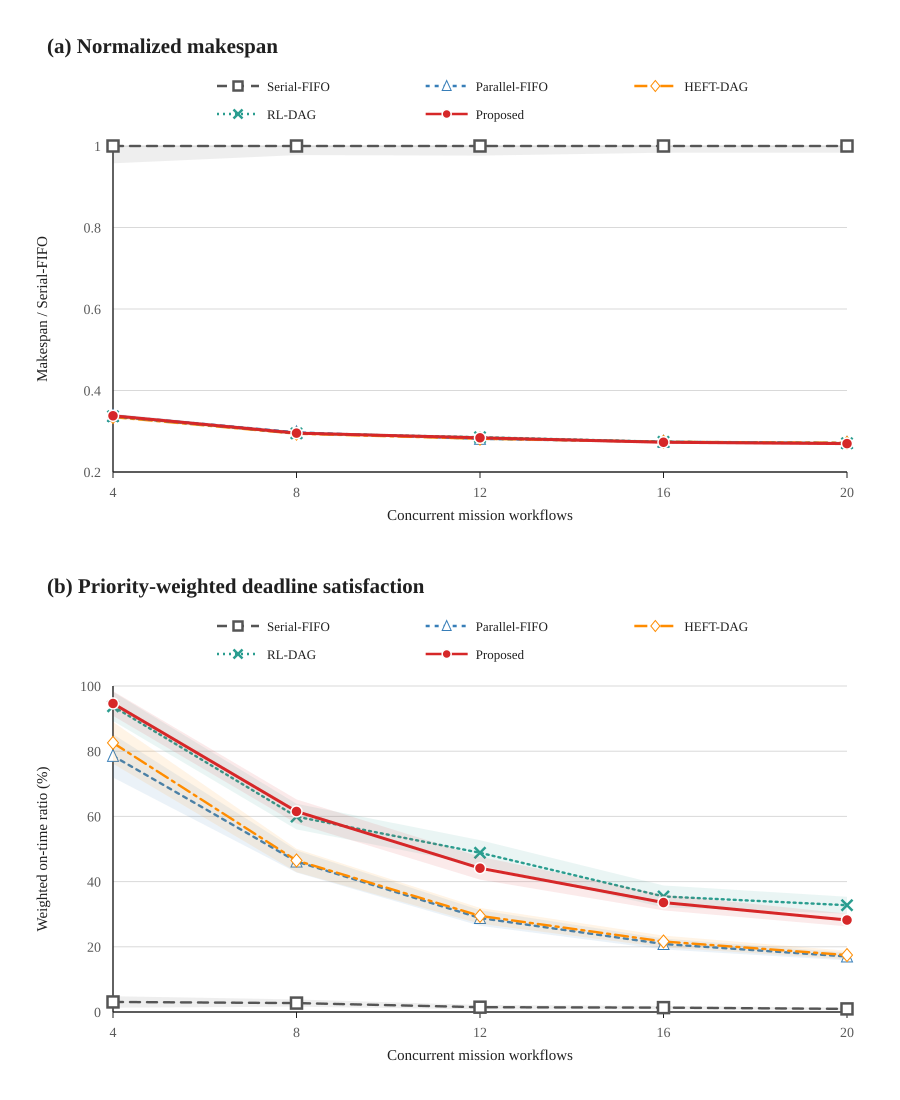
\includegraphics[width=\columnwidth]{figures/scheduler_scalability.png}
\caption{Scheduling scalability under increasing concurrent workflows.}
\label{fig:scalability}
\end{figure}

Fig.~\ref{fig:scalability}(a) shows that all parallel DAG policies reduce
makespan substantially relative to serial invocation. At 20 concurrent
workflows, the normalized makespans of Parallel-FIFO, HEFT-DAG, RL-DAG, and
the proposed method are 0.271, 0.272, 0.271, and 0.270, respectively. Thus,
dependency parallelism supplies most of the total completion-time gain. The
proposed method is not designed to minimize makespan alone; rather, it
preserves comparable completion time while reserving ordering capacity for
deadline-aware recovery and auditable execution.

The difference among parallel policies becomes visible when deadlines are
weighted by clinical urgency. At 20 workflows, HEFT-DAG attains 17.47\%
weighted on-time service, RL-DAG attains 32.8\%, and the proposed scheduler
attains 28.2\%, a 61.2\% relative improvement over HEFT-DAG. Serial-FIFO
reaches only 0.95\%. The result indicates that pure task-level
critical-path rank is insufficient when multiple medical workflows compete
for the same service capacity. RL-DAG is a strong nominal ordering baseline;
the recovery-controlled experiments below therefore separate learned ranking
from capability recovery.

\begin{figure}[t]
\centering
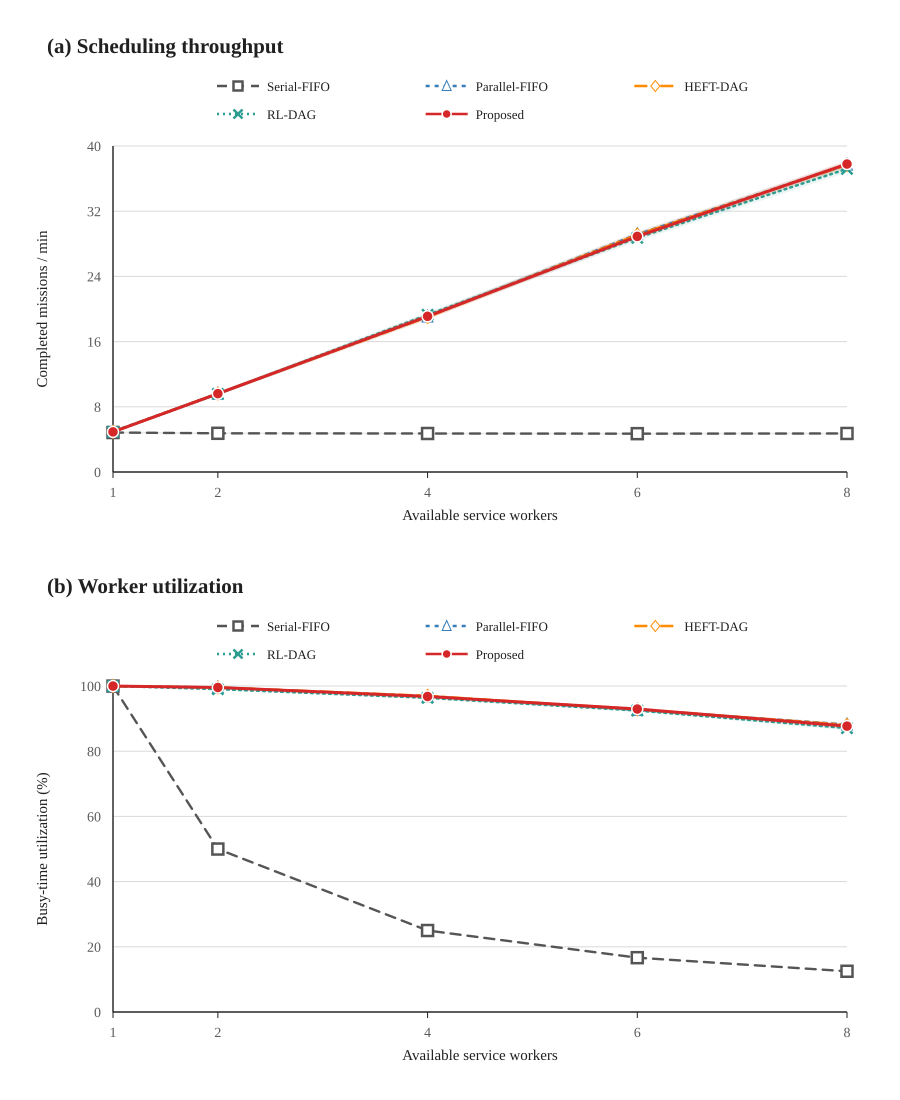
\includegraphics[width=\columnwidth]{figures/scheduler_resource_efficiency.png}
\caption{Resource efficiency under increasing service-worker capacity.}
\label{fig:resources}
\end{figure}

As shown in Fig.~\ref{fig:resources}, throughput scales from approximately
5 completed missions/min with one worker to 37.79 missions/min with eight
workers for the proposed method. The parallel schedulers retain about
87--97\% worker utilization over the tested range. Serial-FIFO intentionally
uses a single execution slot, so its utilization relative to total
provisioned capacity falls to 12.5\% at eight workers.

\subsection{Failure Robustness and Ablation}

\begin{figure}[t]
\centering
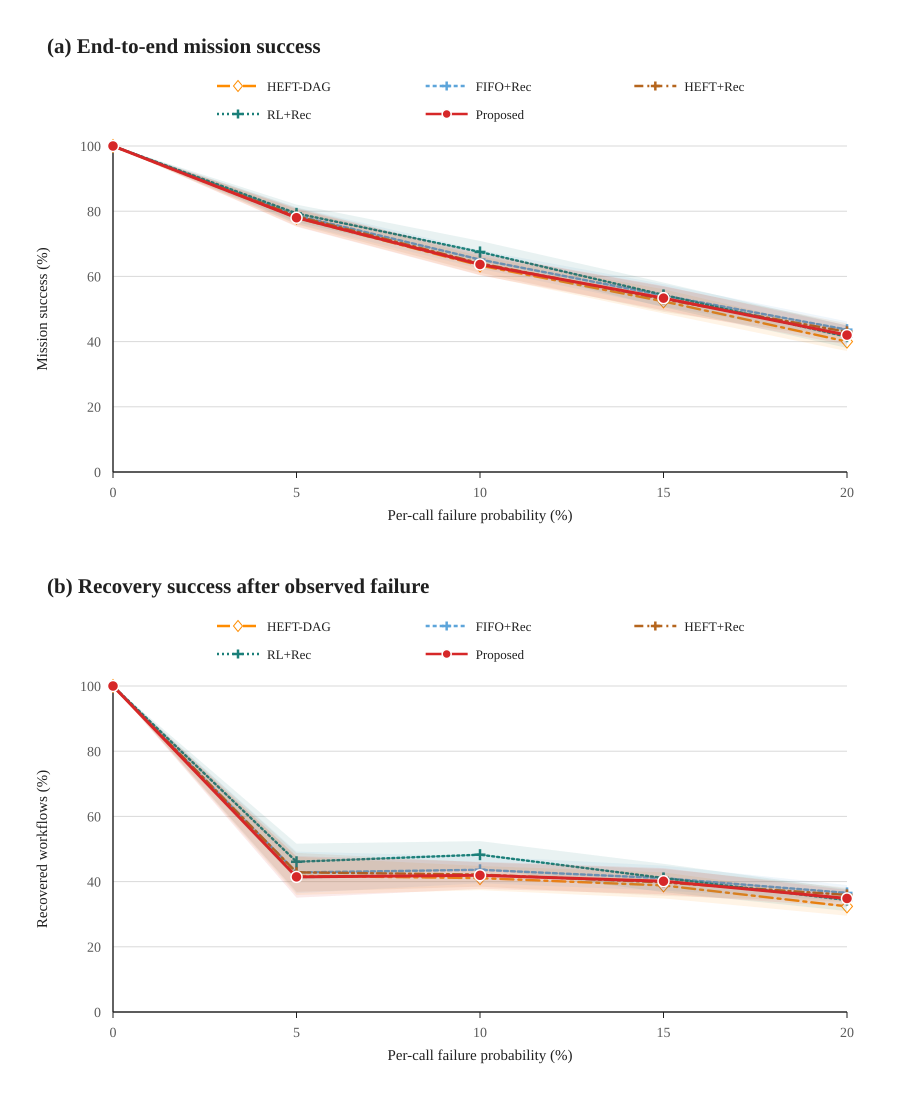
\includegraphics[width=\columnwidth]{figures/scheduler_robustness.png}
\caption{Failure robustness under increasing per-call failure probability.}
\label{fig:robustness}
\end{figure}

Fig.~\ref{fig:robustness} separates recovery effects from ordering effects.
At a 20\% per-call failure probability, HEFT-DAG without fallback succeeds in
40.0\% of missions. Adding the same capability recovery to FIFO, HEFT, and
RL ordering increases raw success to 43.7\%, 43.0\%, and 41.5\%,
respectively. The proposed scheduler reaches 42.0\% raw success, confirming
that raw completion is primarily driven by whether recovery is available.
The ordering contribution appears in the deadline-weighted metric: the
proposed method reaches 19.8\% priority-weighted on-time service, compared
with 18.5\% for HEFT-DAG+Recovery and 19.0\% for RL-DAG+Recovery. Thus, the
proposed policy trades a small amount of raw-completion optimality for better
clinical deadline preservation under the same recovery mechanism.

\begin{figure}[t]
\centering
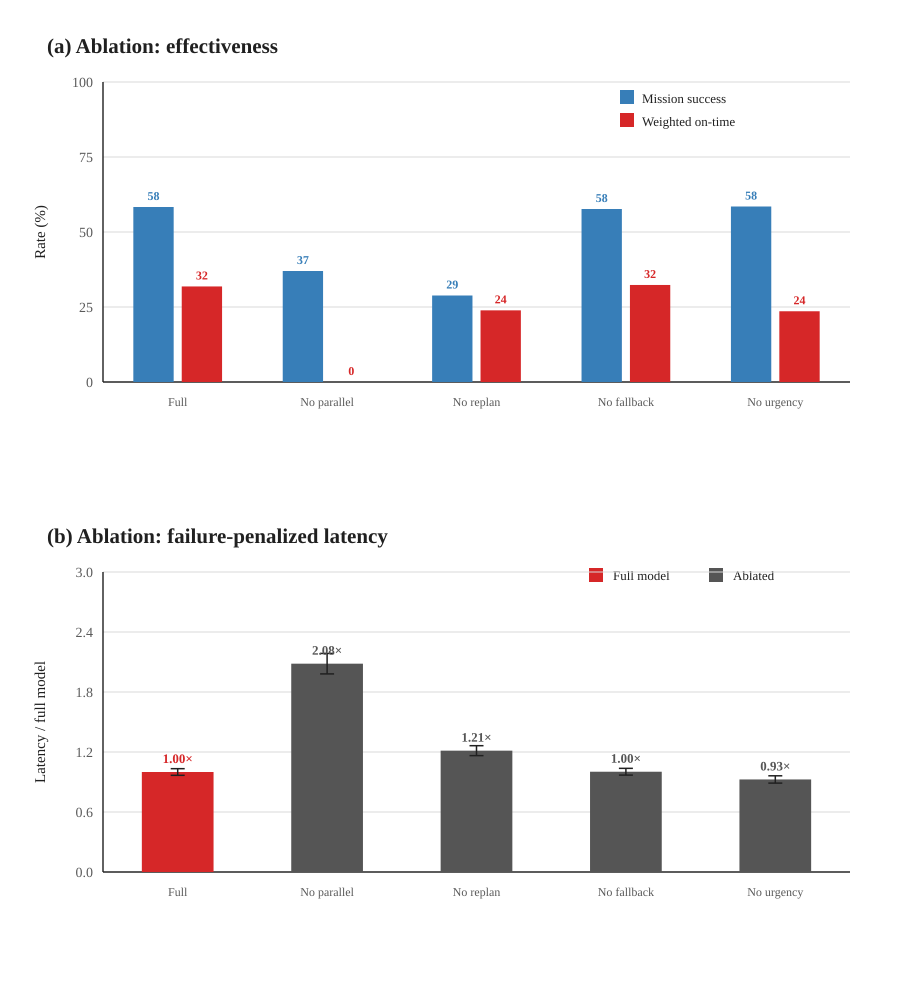
\includegraphics[width=\columnwidth]{figures/scheduler_ablation.png}
\caption{Mechanism ablation under combined workflow load and service failure.}
\label{fig:ablation}
\end{figure}

The ablation in Fig.~\ref{fig:ablation} isolates the source of these gains.
Removing parallelism lowers mission success from 58.3\% to 37.0\%, eliminates
weighted on-time service, and doubles penalized latency. Removing replanning
lowers mission success to 28.8\% and increases penalized latency by
1.21$\times$. Removing fallback has a small average effect in this aggregate
because only specific capability failures activate it and the deadline guard
can terminate late recoveries, but fallback remains important in the
scenario-level traces. Removing urgency priority leaves success nearly
unchanged while reducing weighted on-time service from 31.8\% to 23.6\%,
confirming that the priority key redistributes capacity toward clinically
important workflows.

\subsection{Joint Load--Failure Pressure Test}

\begin{table}[t]
\centering
\caption{Weighted Deadline Gain over HEFT-DAG (Percentage Points)}
\label{tab:pressure}
\footnotesize
\begin{tabular}{c|ccc}
\toprule
\textbf{Failure} & \textbf{4 workflows} & \textbf{12 workflows} &
\textbf{20 workflows}\\
\midrule
0\%  & +10.1 & +9.6  & +11.8\\
10\% & +17.2 & +11.3 & +3.4\\
20\% & +10.0 & +6.4  & +1.8\\
\bottomrule
\end{tabular}
\end{table}

Table~\ref{tab:pressure} summarizes the interaction between queueing pressure
and unreliable services. The proposed method improves weighted deadline
satisfaction in every tested cell. Across the full grid, the largest gain is
18.5 percentage points for four workflows at a 5\% failure probability.
Even at 20 workflows and a 20\% failure probability, the gain remains
positive at 1.8 points. Benefits are largest when sufficient capacity remains
for recovery actions to affect which urgent workflows complete before their
deadlines. The complete annotated heatmap is included with the reproducible
paper artifacts.

\subsection{Correlated Failures and Geographic Validation}

\begin{figure}[t]
\centering
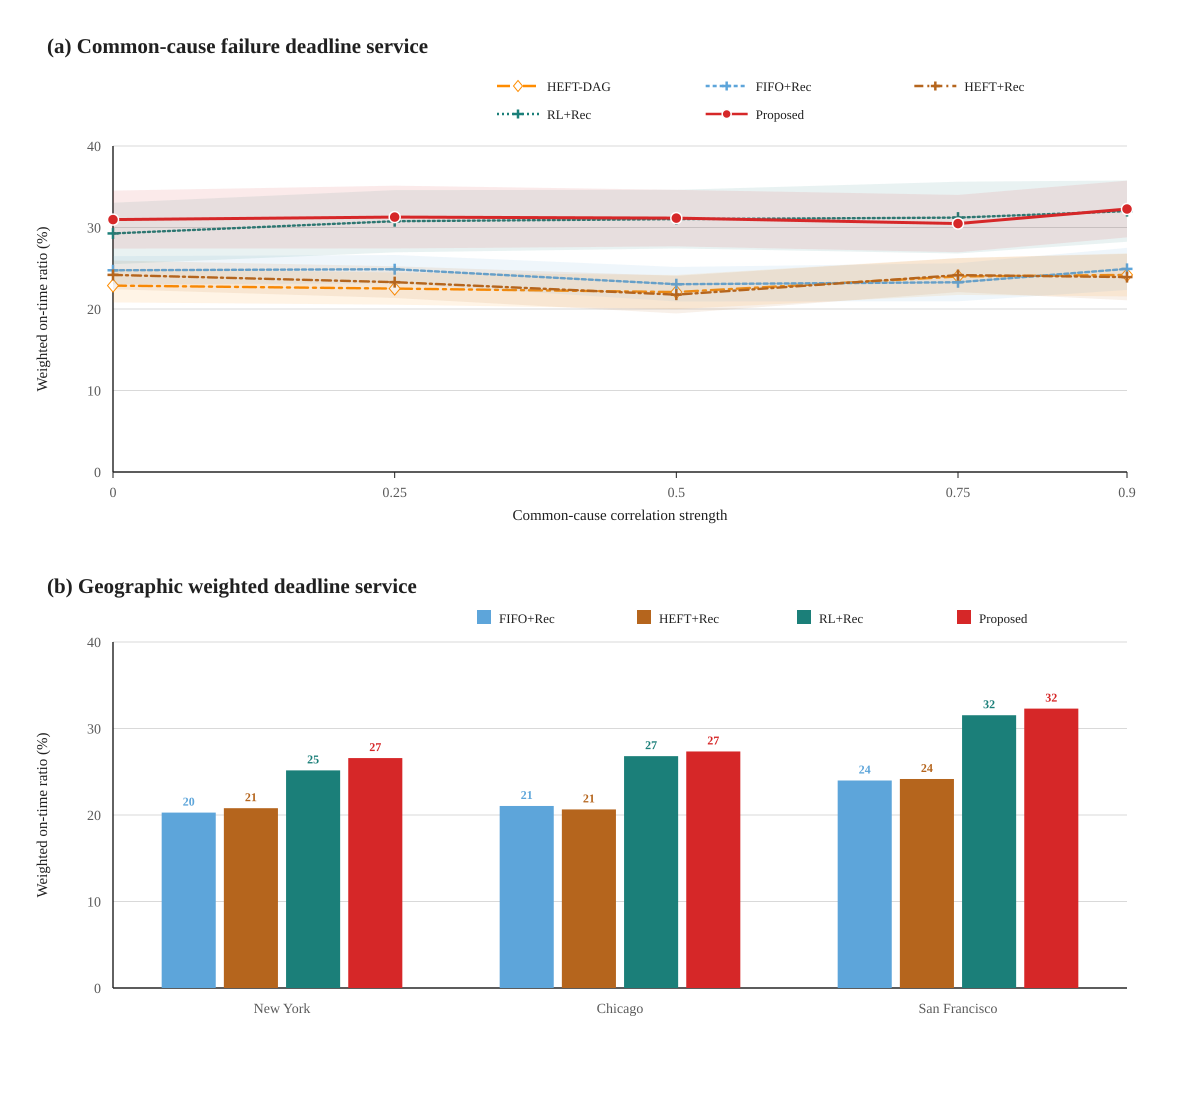
\includegraphics[width=\columnwidth]{figures/scheduler_correlated_geography.png}
\caption{Priority-weighted deadline service under common-cause failures and
geographically parameterized city scenarios.}
\label{fig:correlated_geo}
\end{figure}

Fig.~\ref{fig:correlated_geo}(a) evaluates the correlated failure model in
\eqref{eq:corrfailure} at a 12\% residual failure probability and plots
priority-weighted deadline service. Under a 0.75 correlation strength,
HEFT-DAG+Recovery attains 24.2\%, RL-DAG+Recovery attains 31.2\%, and the
proposed method attains 30.5\%. The underlying raw-success results show that
recovery-controlled FIFO, HEFT, and RL ordering reach 50.0\%, 48.2\%, and
49.8\%, respectively, while the proposed method reaches 47.3\%. At a more
severe 0.90 correlation strength, the proposed method obtains the highest
weighted deadline service, 32.3\%, narrowly above RL-DAG+Recovery at 32.0\%.
These results show that recovery availability drives raw completion under
common-cause failures, while ordering determines which clinically urgent
workflows survive the deadline pressure.

Fig.~\ref{fig:correlated_geo}(b) reports the three city profiles in
Table~\ref{tab:geo} with 10\% residual failures and 0.70 correlated shocks.
The proposed method does not maximize raw success in these profiles; for
example, FIFO+Recovery reaches 61.0\% success in San Francisco. However, the
proposed method obtains the highest priority-weighted on-time rate in all
three cities: 26.6\% in New York, 27.3\% in Chicago, and 32.3\% in San
Francisco. RL-DAG+Recovery is the closest learned baseline, with 25.2\%,
26.8\%, and 31.5\%, respectively.
These geographic experiments do not replace operational flight logs; rather,
they verify that the orchestration conclusions persist when distance, wind,
and wet-weather parameters are tied to concrete urban medical-delivery
settings.

\section{Discussion and Limitations}

The recovery-controlled baselines clarify the source of improvement. Adding
capability recovery to FIFO, HEFT, or RL ordering improves raw completion
because more failed services can be repaired or replaced. The proposed
scheduler should therefore not be interpreted as a universal raw-success
maximizer. Its contribution is the coupling of active-recovery priority,
clinical urgency, and critical-path rank so that limited service capacity is
spent on workflows that can still preserve medical deadline value.

The study has four limitations. First, the recent DRL-LLM, temporal-logic
trajectory, CoordField, air-ground, and medical scheduling services are
represented by integrated algorithm-service models rather than exact
reproductions of published neural weights or commercial solvers. Second, the
benchmark measures orchestration with synthetic service-time distributions,
not real flight operations. Third, the correlated failure model is a
common-cause stress generator rather than a calibrated outage model learned
from radar, communication, or airspace-management logs. Fourth, the
geographic profiles use real coordinates and fixed weather summaries, but
not certified UAV corridors, regulatory geofences, or historical medical
demand traces.


\section{Conclusion}

This paper presented a capability-aware multi-agent framework for
orchestrating heterogeneous low-altitude emergency medical delivery
services. The system transforms mission semantics into a dependency DAG,
executes compatible services in parallel through a typed interface, ranks
workflows by deadline, urgency, and critical path, and recovers through
capability-specific retry, waiting, fallback, and skip policies. Functional
scenarios demonstrate weather, airspace, and fleet-resource recovery.
Reproducible simulation shows that the proposed scheduler preserves the
makespan benefits of DAG parallelism while disentangling recovery-driven
raw success from priority-driven deadline service. Recovery-controlled
baselines show that fallback availability explains much of the completion
gain, whereas the proposed ordering improves clinically weighted deadline
service under heavy failure and geographic stress.
The results support treating multi-agent scheduling and service recovery as
first-class components of low-altitude logistics systems, rather than as
implementation details around a route optimizer.

\bibliographystyle{IEEEtran}
\bibliography{references}

\end{document}
